%xelatex
\documentclass{article}

\usepackage[T2A]{fontenc}
\usepackage[english,ukrainian]{babel}
\usepackage{fontspec}
\setmainfont{Nimbus Roman}
\usepackage{graphicx}
\usepackage[a4paper,margin=0.5in]{geometry}
\pagestyle{empty}

\usepackage{pgfplots}% loads the package tikz
\pgfplotsset{compat=1.18}
\usetikzlibrary{intersections}
\usepackage{wrapfig}
\usepackage{pdfpages}
\usepackage{subfiles}

\begin{document}
\includepdf[pages=-]{14title.pdf}
{\fontsize{14}{16.2}\selectfont

\section*{Мета роботи}
використовуючи оборотний маятник, визначити прискорення
вільного падіння.

\section*{Прилади та обладнання}
оборотний маятник, міліметрова лінійка, секундомір.

\section*{Опис вимірювального пристрою, виведення
робочої формули}

\begin{figure}[h]
	\centering
	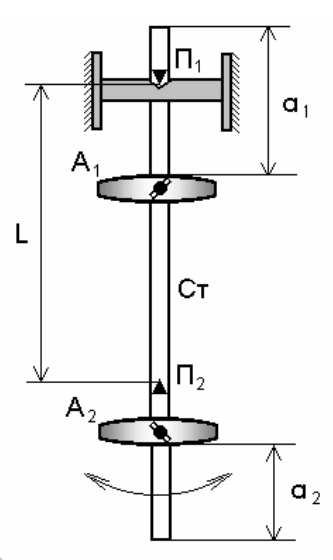
\includegraphics[width=3cm]{~/mayatnik.png}
	\caption{оборотний маятник}
\end{figure}

     Застосований в даній роботі оборотний маятник складається із
стрижня  Ст, що має прямокутний переріз та вантажів  А$_1$ і  А$_2$, які
можна  переміщати  вздовж  стрижня.  На  невеликих  відстанях  від
кінців стрижня закріплені опорні призми П$_1$ і П$_2$, за  горизонтальні
ребра яких маятник можна почергово підвішувати на кронштейн К.
Під  дією  сили  земного  тяжіння  маятник  може  здійснювати
гармонічні коливання.

\medskip

       Якщо переміщенням вантажу  А2 досягати такого взаємного
розташування вантажів А$_1$ і А$_2$ , що періоди коливань маятника при
підвішуванні за призми  П$_1$ і П$_2$  зрівнюються між собою, то зведена
  довжина фізичного маятника дорівнюватиме відстані між
опорними ребрами призм: Lзв = L.  Визначивши експериментально
період коливань маятника Т для вказаного розташування  вантажів,
при відомій величині L з формули

$$T=2\pi\sqrt{\frac{L}{g}}$$

              знайдемо:

$$g=\frac{4\pi^2L}{T^2}.$$

\section*{Задані величини}
Зведена довжина маятника $L=(100\pm0.05)$ см або $(1\pm0.05)$ м.

\section*{Фізичні величини, які вимірюються прямим способом}
Час 10 повних коливань маятника.

\bigskip

\section*{\centering{Таблиця результатів вимірювань}}

\renewcommand{\arraystretch}{1.3}
\begin{center}
\begin{tabular}{|c| c| c| c| c| c| c|}
	\hline
	$\alpha_2$, см & 12 & 14 & 16 & 18 & 20 & 22\\
	\hline
	$t_1$, с (П$_1$) & 20.34 & 20.27 & 20.19 & 19.53 & 19.42 & 19.20\\
	\hline
	$T_1$, с & 2.034 & 2.027 & 2.019 & 1.953 & 1.942 & 1.920\\
	\hline
	$t_2$, с (П$_2$) & 20.49 & 20.37 & 20.27 & 19.41 & 19.35 & 19.18\\
	\hline
	$t_2$, с & 2.049 & 2.037 & 2.027 & 1.941 & 1.935 & 1.918\\
	\hline
\end{tabular}

\end{center}
}

{\fontsize{14}{16.2}\selectfont
\begin{center}
\section*{Графіки залежностей}
\subfile{plot.tex}

\section*{Обчислення шуканої величини за робочою формулою}
	Графіки перетнулися в точці (16.4,1.99), отже період
	коливань маятника дорівнює 1.99 с. Підставимо це
	значення у робочу формулу і знайдемо g:

	$$g=\frac{4\pi^2L}{T^2}=\frac{4\cdot3.14^2\cdot1}{1.99^2}=
	9.9589\textrm{, [м/с$^2$]}$$


\section*{Обчислення похибок}

	$\Delta T = \frac{\Delta t}{10} = \pm \frac{0.2}{10} = \pm 0.02 \textrm{ [с].}$
	\medskip

	$\Delta \pi = 0.005$

	$\Delta L =  0.05\textrm{ см або 0.0005 м}$

	\bigskip

	Логарифмуємо робочу формулу:
	$\ln\left(\frac{4\pi^2L}{T^2}\right)=\ln4 + \ln\pi^2
	+ \ln L - \ln T^2,$
	і диференціюємо отриманий вираз:
	$d(\ln4 + \ln\pi^2
	+ \ln L - \ln T^2) =
	2\frac{d\pi}{\pi}+\frac{dL}{L}- 2\frac{dT}{T}.$
	Отже, відносна похибка:
	$$\delta g = \frac{\Delta g}{g} = 2\frac{\Delta\pi}{\pi}+\frac{\Delta L}{L}+
	2\frac{\Delta T}{T} = \frac{2 \cdot 0.005}{3.14}+\frac{0.0005}{1}+
	\frac{0.02}{1.99} = 0.013 [\%].$$

	Абсолютна похибка:
	$$\Delta g = g\cdot\delta g = 9.9589 \cdot 0.013\% = 0.0012\textrm{ [м/с$^2$].}$$

\section*{Запис кінцевого результату}

	$$g=(9.95\pm0.0012) \textrm{ м/с$^2$.}$$

\end{center}
\section*{Аналіз кінцевих результатів та висновки}

	Виконуючи цю роботу, я навчився використовувати оборотний
	маятник для знаходження величини прискорення вільного
	падіння.

\vspace{350pt}
Оцінка за виконання роботи:
\smallskip

\renewcommand{\arraystretch}{4}
\begin{tabular}{|c|c|c|}
	\hline
	\hspace{15pt} Допуск \hspace{15pt} & \hspace{15pt} Захист \hspace{15pt}
	& \hspace{15pt} Дата виконання \hspace{15pt}\\
	\hline
	 &  & \\
	\hline

\end{tabular}

\bigskip

	\begin{flushright}
		Підпис викладача:\line(1,0){70}\hspace{100pt}\hphantom{1pt}
	\end{flushright}
	}

\end{document}
